\documentclass[]{article}
\usepackage{amsmath}
\usepackage{amssymb}
\usepackage{verbatim} %con verbatim escribes bloques de texto con letra mono.
\usepackage{graphicx} %para insertar imagenes, cuando meta yo una usa el codigo de ejemplo
\usepackage{listings}
\usepackage{fullpage}
\usepackage{color}
\usepackage{fancyvrb}
\usepackage[spanish]{babel}
\usepackage[utf8]{inputenc} %Para usar acentos directamente en latex
\usepackage{hyperref} %Para que el indice tenga hiperenlaces y si quieres poner los tuyos
\hypersetup{%
	pdfborder = {0 0 0}
}

\definecolor{mygreen}{rgb}{0,0.6,0}
\definecolor{mygray}{rgb}{0.5,0.5,0.5}
\definecolor{mymauve}{rgb}{0.58,0,0.82}

%Para insertar código: crea un recuadro con texto mono y lineas enumeradas. Puedes referenciar un fichero y no copiar y pegar aquí.
\lstset{ %
	backgroundcolor=\color{white},   % chohttp://xdxd.com/ose the background color; you must add \usepackage{color} or \usepackage{xcolor}
	basicstyle=\footnotesize,        % the size of the fonts that are used for the code
	breakatwhitespace=false,         % sets if automatic breaks should only happen at whitespace
	breaklines=true,                 % sets automatic line breaking
	captionpos=b,                    % sets the caption-position to bottom
	commentstyle=\color{mygreen},    % comment style
	frame=single,                    % adds a frame around the code
	keepspaces=true,                 % keeps spaces in text, useful for keeping indentation of code (possibly needs columns=flexible)
	numbers=left,                    % where to put the line-numbers; possible values are (none, left, right)
	numbersep=5pt,                   % how far the line-numbers are from the code
	numberstyle=\tiny\color{mygray}, % the style that is used for the line-numbers
	rulecolor=\color{black},         % if not set, the frame-color may be changed on line-breaks within not-black text (e.g. comments (green here))
	showspaces=false,                % show spaces everywhere adding particular underscores; it overrides 'showstringspaces'
	showstringspaces=false,          % underline spaces within strings only
	showtabs=false,                  % show tabs within strings adding particular underscores
	stepnumber=1,                    % the step between two line-numbers. If it's 1, each line will be numbered
	stringstyle=\color{mymauve},     % string literal style
	tabsize=4,
	inputencoding=utf8,
	title=\lstname                   % show the filename of files included with \lstinputlisting; also try caption instead of title
}

\usepackage{pdfpages}

\title{Computación Móvil}
\author{José Luis Cánovas Sánchez - 48636907A\\Ezequiel Santamaría Navarro - 20096517Z}

\begin{document}

\maketitle


\tableofcontents

\section{Manual de usuario}

\section{Diseño e implementación}

Telefun se basa en un servidor centralizado que almacena a los usuarios y sus datos, lista de contactos y conversaciones. Los clientes se conectan al servidor por HTTP/REST, usando para identificarse un token único para cada usuario. Esto permite que las conversaciones se puedan ver por cualquier app que implemente los mensajes HTTP/REST o por un navegador web.

Por esta estructura de servidor centralizado y acceso a las conversaciones por múltiples dispositivos, llamamos a la aplicación \textit{Telefun}, al ser más del estilo de \textit{Telegram} que de \textit{Whatsapp}.

Se detallan las características de la app y del servidor en las secciones siguientes, donde se irán mencionando cómo se han implementado las mejoras:
\begin{itemize}
	\item Geo-localización de usuarios.
	\item Persistencia de conversaciones y de la agenda de contactos del usuario.
	\item Recepción de notificaciones cuando lleguen mensajes, aunque la aplicación no se encuentre en primer plano.
	\item Securización de los mensajes intercambiados.
\end{itemize}

\subsection{Arquitectura de la aplicación}


\subsubsection{Diagrama de clases}

Se incluye en la página a continuación el diagrama de clases de la implementación de la app. Por razones de espacio, la página en pdf es más larga que el resto y se recomienda verlo por ordenador.

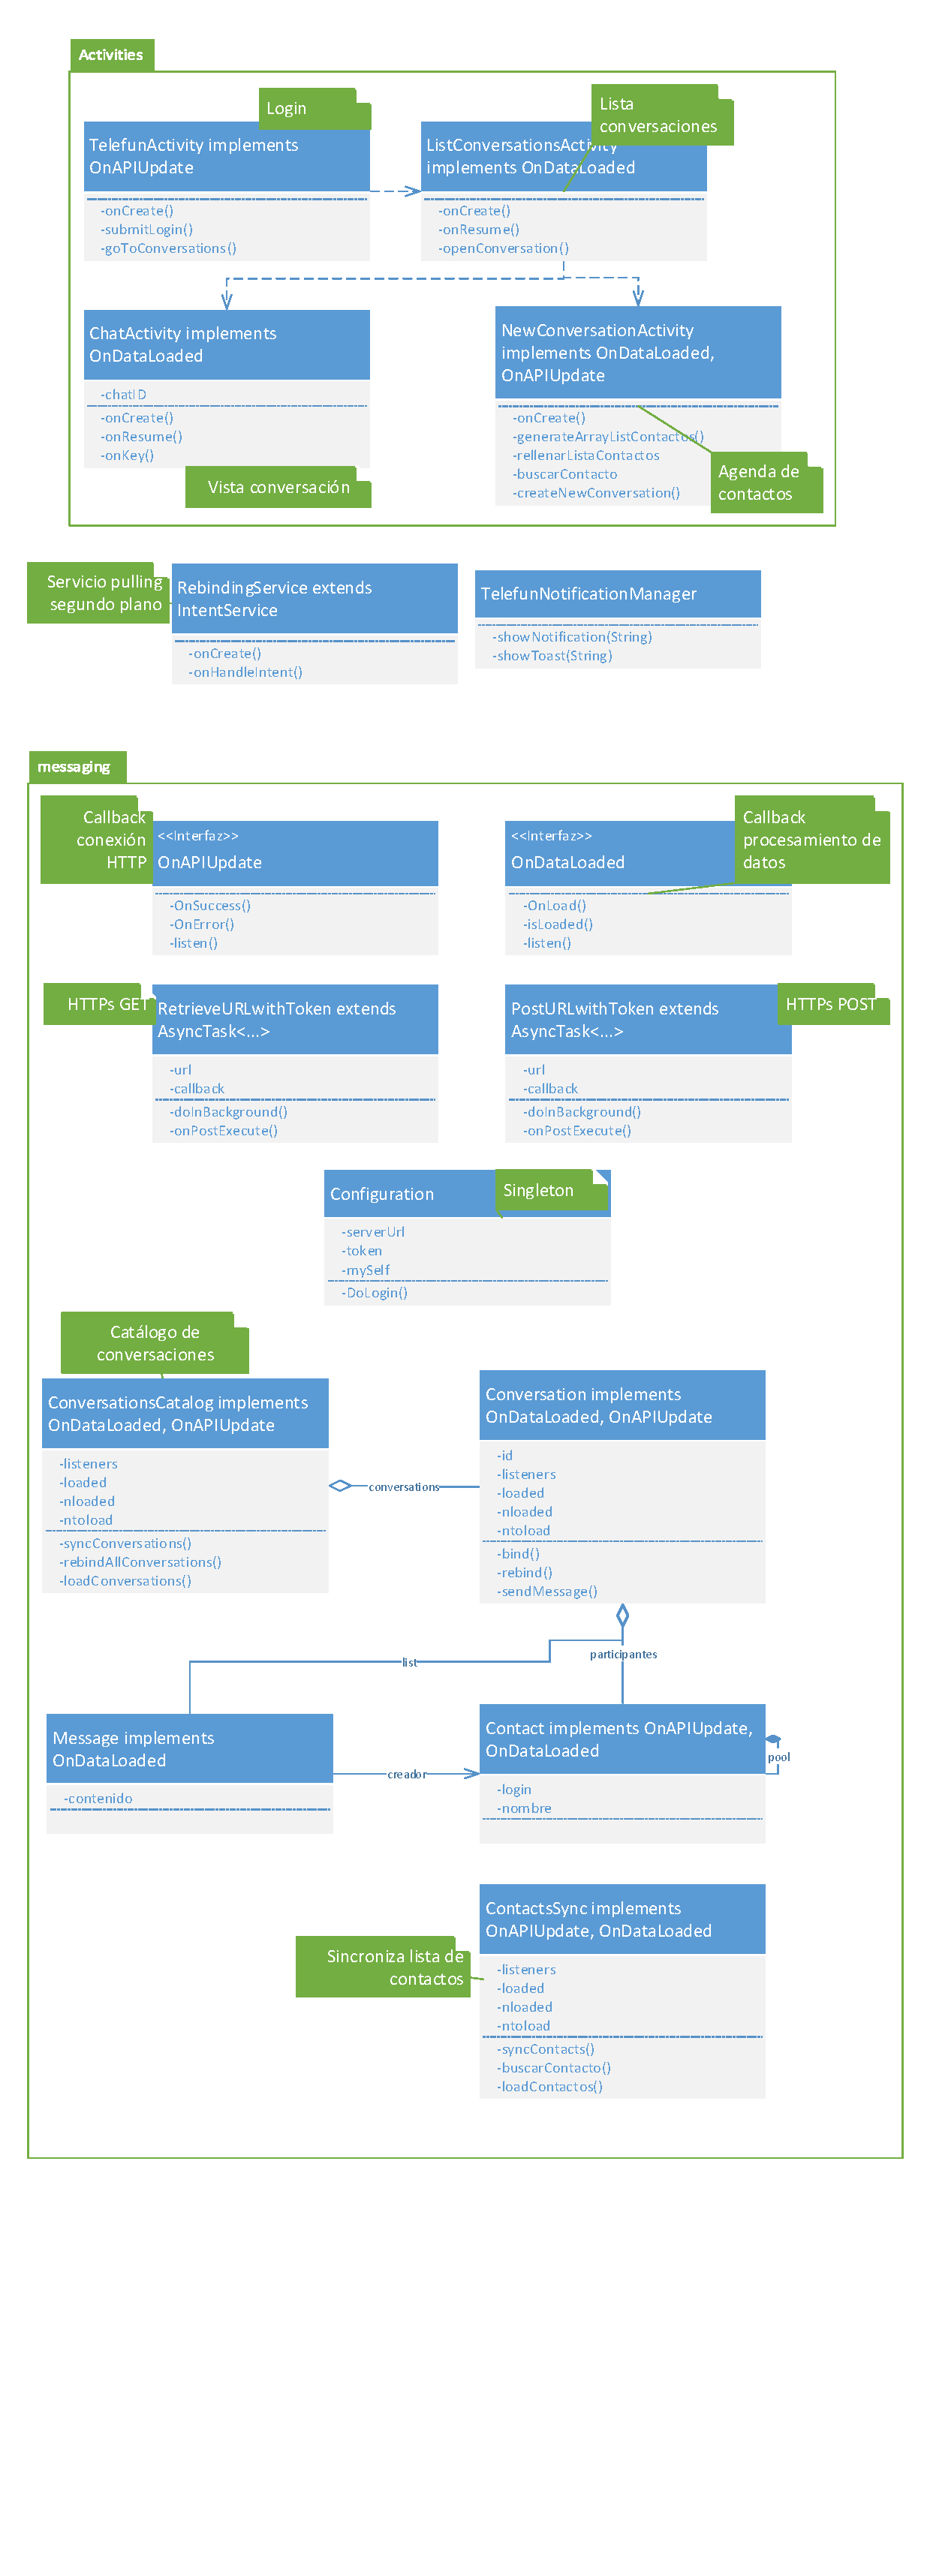
\includepdf[pages=-,fitpaper=true]{DiagramaClases.pdf}

\subsection{Servidor REST}

El servidor guarda en estructuras JSON toda la información: de los contactos, su nombre, login único y contraseña, lista de contactos y conversaciones. Para poder hacer llamadas HTTP/REST válidas, los mensajes GET y POST deben ir acompañados de una Cookie \textit{token}, con el valor del token único generado en el último inicio de sesión del usuario con su login y contraseña.

Para conseguir el token, un usuario debe hacer una petición del tipo

 \textit{urlServidor/usuarios/:usuario/token?password=:contraseña}
 
  donde \textit{:usuario} se debe sustituir por el login único del usuario, y \textit{:contraseña} por su contraseña. Esta llamada devuelve un token en forma de \textit{Set-Cookie} que se debe guardar en la app para evitar tener que insertar de nuevo el login y contraseña. Si se realiza el inicio de sesión en otro dispositivo, se genera un nuevo token y por seguridad no se aceptan los token antiguos, por lo que en la app se cerrará la sesión.

\hfill

Como servidor estamos usando el servicio \textit{Bluemix} de IBM, el cual nos automatiza el conseguir un certificado para que funcione el HTTPS sin tener que crear nuestra propia PKI.

\hfill

Al usar \textbf{HTTPS} junto a los \textbf{token} de usuario, en el intercambio de todos los mensajes con el servidor, conseguimos otra de las funcionalidades, \textbf{\textit{securización de los mensajes intercambiados}}. Y por el hecho de guardar todo en el servidor, conseguimos la \textbf{\textit{persistencia de conversaciones y de contactos del usuario}} no sólo en la app, sino en todos los clientes donde iniciemos sesión.

\hfill

Una vez hemos iniciado sesión y obtenemos el token, estos son los mensajes que se pueden intercambiar con el servidor:

\begin{itemize}
	\item get /usuarios/:usuario
	
	Devuelve en JSON los datos de contacto públicos de un usuario. En concreto su nombre (\textit{José Luis} por ejemplo), y su login único (\textit{joseluis}).
	
	\item get /usuarios/:usuario/token?password=:contraseña
	
	Si los datos de :usuario y :contraseña son correctos, devuelve en la respuesta HTTP/S una cabecera Set-Cookie con un nuevo token generado para :usuario.
	
	\item get /conversaciones
	
	Devuelve un JSON con la lista de identificadores de conversaciones donde participa el usuario que corresponde al token.
	
	\item get /conversaciones/:id
	
	Devuelve en JSON la conversación con número de identificación :id si el token de la petición corresponde a algún participante de la misma. Esto evita poder leer conversaciones ajenas.
	
	\item get /contactos
	
	Devuelve un JSON con la lista de logins únicos de la lista de contactos del usuario identificado por el token. Así cuando un usuario inicia sesión en una app, recupera su lista de contactos.
	
	\item post /conversaciones/:id/mensaje
	
	Crea un nuevo mensaje en una conversación, con autor el usuario asociado al token, y mensaje el texto que se envíe en el cuerpo de la petición HTTP.
	
	\item post /usuarios/:usuario/ %TODO: Corregir con la contraseña
	
	Permite crear nuevos usuarios en el sistema. En principio existe un formulario web donde realizar el registro, y una vez realizado, se podrá iniciar sesión como se ha explicado antes.
	
	%TODO: añadir nuevas llamadas.
	
\end{itemize}


El servidor está escrito en JavaScript, y corre sobre NodeJS. Esto facilita enormemente la creación del protocolo HTTP/REST y manejar estructuras JSON, propias del lenguaje.



\end{document}
